\documentclass[11pt,a4paper]{article}
\usepackage[T1]{fontenc}
\usepackage{lmodern}
\usepackage[margin=2cm]{geometry}
\usepackage{booktabs,array,graphicx,float,caption,amsmath,longtable}
\usepackage[hidelinks]{hyperref}
\usepackage{setspace}
\setstretch{1.12}
\captionsetup{font=small,labelfont=bf,justification=raggedright,singlelinecheck=false}
\setlength{\parindent}{0pt}\setlength{\parskip}{6pt}
\newcommand{\bestname}{LGBM-FEAT}
\newcommand{\bestacc}{0.548}
\newcommand{\bestfone}{FUSION-MLP}
\newcommand{\bestfoneval}{0.438}
\newcommand{\bestmild}{ECGF-linear}
\newcommand{\bestmildval}{0.282}


\begin{document}
\begin{center}
{\LARGE\bfseries TRAIN100 Results}\\[4pt]
{\large Every model trained to (nearly) 100\,\% training accuracy: accuracy, F1, recall, confusion matrices and model structure}\\[6pt]
{\small Four-class LVEF classification from 12-lead ECG printouts. Development data: 837 ECGs, patient-grouped 5-fold cross-validation $\times$ 3 repeats.\\
The locked test set was not used. EchoNext was used only on the owner's laptop (Section~\ref{sec:echonext}).}
\end{center}

\tableofcontents

\section{What was done}
Every model of the project that could be retrained was trained again, with no early stopping, no weight decay, no augmentation and as many epochs or iterations as it needed, until its training accuracy reached (nearly) 100\,\%. It was then scored on the same held-out folds as the original early-stopped model. The rules were declared before any run (\texttt{AMENDMENT\_TRAIN100.md}, branch \texttt{research/train100}).

\textbf{Metrics.} \emph{Held-out accuracy}: share of held-out ECGs classified correctly (four classes). \emph{Macro-F1}: mean of the four per-class F1 scores (F1 = harmonic mean of precision and recall), so every class counts equally. \emph{Mild F1}: F1 of the hardest class. \emph{Balanced accuracy}: mean of the four recalls. \emph{Recall}: share of each true class found.

\textbf{In one sentence.} Every flexible model now fits its training data perfectly, but none becomes reliably better on new patients: the best four-class accuracy is \bestname{} with \bestacc, the best macro-F1 \bestfone{} with \bestfoneval{} and the best Mild F1 \bestmild{} with \bestmildval, all at or below the early-stopped originals.

\section{Main models ranked by held-out accuracy}
\begin{table}[htbp]
\centering
\caption{Main models trained to (nearly) 100\,\% training accuracy, ranked by held-out accuracy (development cross-validation, 5 folds $\times$ 3 repeats, 837 ECGs). Held-out accuracy: mean of the 15 test folds with the corrected 95\,\% CI. Macro-F1, Mild F1, balanced accuracy and recall: from the confusion matrix pooled within each repeat, averaged over the 3 repeats. Rec. = recall of Normal, Mild, Moderate and Severe. $^{\dagger}$ Selective: scored on the 48\,\% of patients it answers.}\label{tab:main_ranked}
\footnotesize
\begin{tabular}{>{\raggedright\arraybackslash\hspace{0pt}}p{\dimexpr 0.045\linewidth-2\tabcolsep\relax}>{\raggedright\arraybackslash\hspace{0pt}}p{\dimexpr 0.165\linewidth-2\tabcolsep\relax}>{\raggedright\arraybackslash\hspace{0pt}}p{\dimexpr 0.200\linewidth-2\tabcolsep\relax}>{\raggedright\arraybackslash\hspace{0pt}}p{\dimexpr 0.080\linewidth-2\tabcolsep\relax}>{\raggedright\arraybackslash\hspace{0pt}}p{\dimexpr 0.070\linewidth-2\tabcolsep\relax}>{\raggedright\arraybackslash\hspace{0pt}}p{\dimexpr 0.070\linewidth-2\tabcolsep\relax}>{\raggedright\arraybackslash\hspace{0pt}}p{\dimexpr 0.065\linewidth-2\tabcolsep\relax}>{\raggedright\arraybackslash\hspace{0pt}}p{\dimexpr 0.065\linewidth-2\tabcolsep\relax}>{\raggedright\arraybackslash\hspace{0pt}}p{\dimexpr 0.065\linewidth-2\tabcolsep\relax}>{\raggedright\arraybackslash\hspace{0pt}}p{\dimexpr 0.065\linewidth-2\tabcolsep\relax}>{\raggedright\arraybackslash\hspace{0pt}}p{\dimexpr 0.085\linewidth-2\tabcolsep\relax}}
\toprule
\textbf{\#} & \textbf{Model} & \textbf{Held-out accuracy [95\,\% CI]} & \textbf{Macro-F1} & \textbf{Mild F1} & \textbf{Bal. acc.} & \textbf{Rec. N} & \textbf{Rec. Mi} & \textbf{Rec. Mo} & \textbf{Rec. S} & \textbf{Training acc.} \\
\midrule
1 & Triage $^{\dagger}$ & 0.696 [0.630, 0.762] & 0.372 & 0.049 & 0.367 & 0.99 & 0.03 & 0.19 & 0.27 & 1.000 \\
\midrule
2 & LGBM-FEAT & 0.548 [0.512, 0.583] & 0.409 & 0.227 & 0.413 & 0.88 & 0.18 & 0.39 & 0.21 & 1.000 \\
3 & FUSION-MLP & 0.538 [0.499, 0.578] & 0.438 & 0.255 & 0.440 & 0.79 & 0.24 & 0.42 & 0.31 & 1.000 \\
4 & ECGF-MLP & 0.536 [0.506, 0.565] & 0.430 & 0.282 & 0.430 & 0.79 & 0.27 & 0.41 & 0.26 & 1.000 \\
5 & C3 & 0.533 [0.496, 0.569] & 0.423 & 0.260 & 0.419 & 0.81 & 0.24 & 0.39 & 0.24 & 0.995 \\
6 & IMG-C3 & 0.532 [0.492, 0.572] & 0.416 & 0.252 & 0.413 & 0.82 & 0.23 & 0.38 & 0.22 & 1.000 \\
7 & C1 & 0.517 [0.477, 0.558] & 0.426 & 0.265 & 0.426 & 0.76 & 0.26 & 0.38 & 0.32 & 1.000 \\
8 & IMG-vote & 0.503 [0.463, 0.544] & 0.416 & 0.275 & 0.415 & 0.72 & 0.28 & 0.39 & 0.27 & 1.000 \\
9 & ECGF-linear & 0.491 [0.451, 0.532] & 0.408 & 0.282 & 0.407 & 0.70 & 0.29 & 0.36 & 0.28 & 1.000 \\
10 & HDRCLIN-LR & 0.486 [0.436, 0.536] & 0.415 & 0.252 & 0.429 & 0.68 & 0.24 & 0.35 & 0.45 & 0.589 \\
11 & HDR-LR & 0.483 [0.432, 0.535] & 0.391 & 0.210 & 0.409 & 0.72 & 0.17 & 0.32 & 0.42 & 0.529 \\
12 & CLIN-LR & 0.442 [0.390, 0.493] & 0.376 & 0.240 & 0.382 & 0.60 & 0.25 & 0.36 & 0.32 & 0.720 \\
\bottomrule
\end{tabular}
\end{table}


\begin{figure}[H]
\centering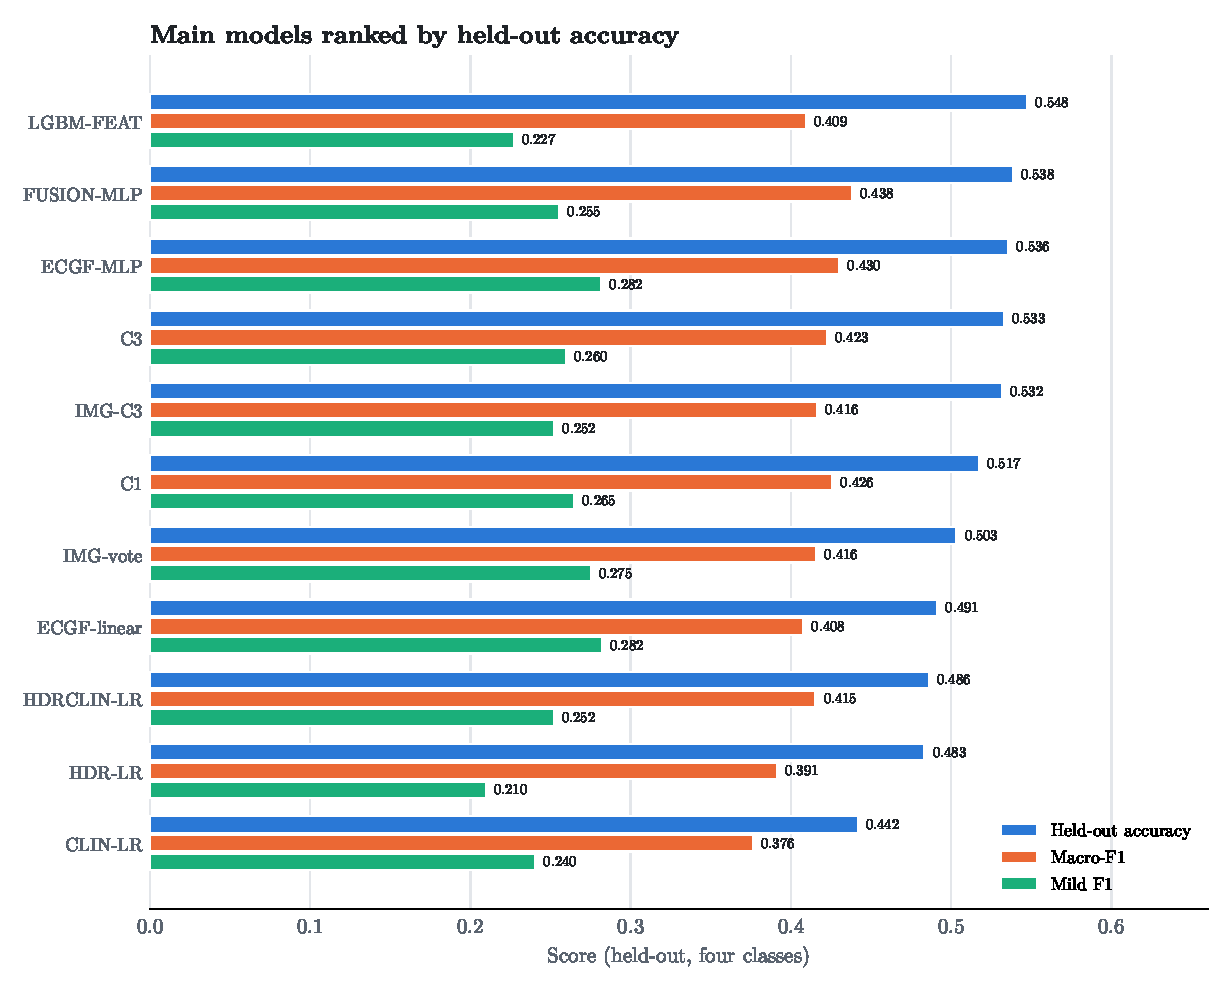
\includegraphics[width=0.86\linewidth]{figures/fig_ranking}
\caption{Held-out accuracy, macro-F1 and Mild F1 of the four-class main models (ranked by accuracy).}
\end{figure}

\section{Compared with the original (early-stopped) models}
\begin{table}[htbp]
\centering
\caption{The same models before (original, early-stopped, report 45) and after training to (nearly) 100\,\%. Change in percentage points. Triage: original macro-F1 and Mild F1 were not recorded in its run summary.}\label{tab:main_vs_original}
\footnotesize
\begin{tabular}{>{\raggedright\arraybackslash\hspace{0pt}}p{\dimexpr 0.160\linewidth-2\tabcolsep\relax}>{\raggedright\arraybackslash\hspace{0pt}}p{\dimexpr 0.280\linewidth-2\tabcolsep\relax}>{\raggedright\arraybackslash\hspace{0pt}}p{\dimexpr 0.280\linewidth-2\tabcolsep\relax}>{\raggedright\arraybackslash\hspace{0pt}}p{\dimexpr 0.280\linewidth-2\tabcolsep\relax}}
\toprule
\textbf{Model} & \textbf{Accuracy: original $\rightarrow$ now (change)} & \textbf{Macro-F1: original $\rightarrow$ now (change)} & \textbf{Mild F1: original $\rightarrow$ now (change)} \\
\midrule
Triage & 0.694 $\rightarrow$ 0.696 (+0.2) & -- $\rightarrow$ 0.372 & -- $\rightarrow$ 0.049 \\
LGBM-FEAT & 0.524 $\rightarrow$ 0.548 (+2.4) & 0.416 $\rightarrow$ 0.409 (-0.7) & 0.228 $\rightarrow$ 0.227 (-0.1) \\
FUSION-MLP & 0.544 $\rightarrow$ 0.538 (-0.6) & 0.440 $\rightarrow$ 0.438 (-0.2) & 0.186 $\rightarrow$ 0.255 (+6.9) \\
ECGF-MLP & 0.542 $\rightarrow$ 0.536 (-0.6) & 0.446 $\rightarrow$ 0.430 (-1.6) & 0.239 $\rightarrow$ 0.282 (+4.3) \\
C3 & 0.561 $\rightarrow$ 0.533 (-2.8) & 0.448 $\rightarrow$ 0.423 (-2.5) & 0.221 $\rightarrow$ 0.260 (+3.9) \\
IMG-C3 & 0.558 $\rightarrow$ 0.532 (-2.6) & 0.441 $\rightarrow$ 0.416 (-2.5) & 0.227 $\rightarrow$ 0.252 (+2.5) \\
C1 & 0.547 $\rightarrow$ 0.517 (-3.0) & 0.455 $\rightarrow$ 0.426 (-2.9) & 0.255 $\rightarrow$ 0.265 (+1.0) \\
IMG-vote & 0.541 $\rightarrow$ 0.503 (-3.8) & 0.450 $\rightarrow$ 0.416 (-3.4) & 0.264 $\rightarrow$ 0.275 (+1.1) \\
ECGF-linear & 0.530 $\rightarrow$ 0.491 (-3.9) & 0.444 $\rightarrow$ 0.408 (-3.6) & 0.266 $\rightarrow$ 0.282 (+1.6) \\
HDRCLIN-LR & 0.501 $\rightarrow$ 0.486 (-1.5) & 0.424 $\rightarrow$ 0.415 (-0.9) & 0.269 $\rightarrow$ 0.252 (-1.7) \\
HDR-LR & 0.489 $\rightarrow$ 0.483 (-0.6) & 0.393 $\rightarrow$ 0.391 (-0.2) & 0.198 $\rightarrow$ 0.210 (+1.2) \\
CLIN-LR & 0.509 $\rightarrow$ 0.442 (-6.7) & 0.417 $\rightarrow$ 0.376 (-4.1) & 0.205 $\rightarrow$ 0.240 (+3.5) \\
\bottomrule
\end{tabular}
\end{table}


\begin{figure}[H]
\centering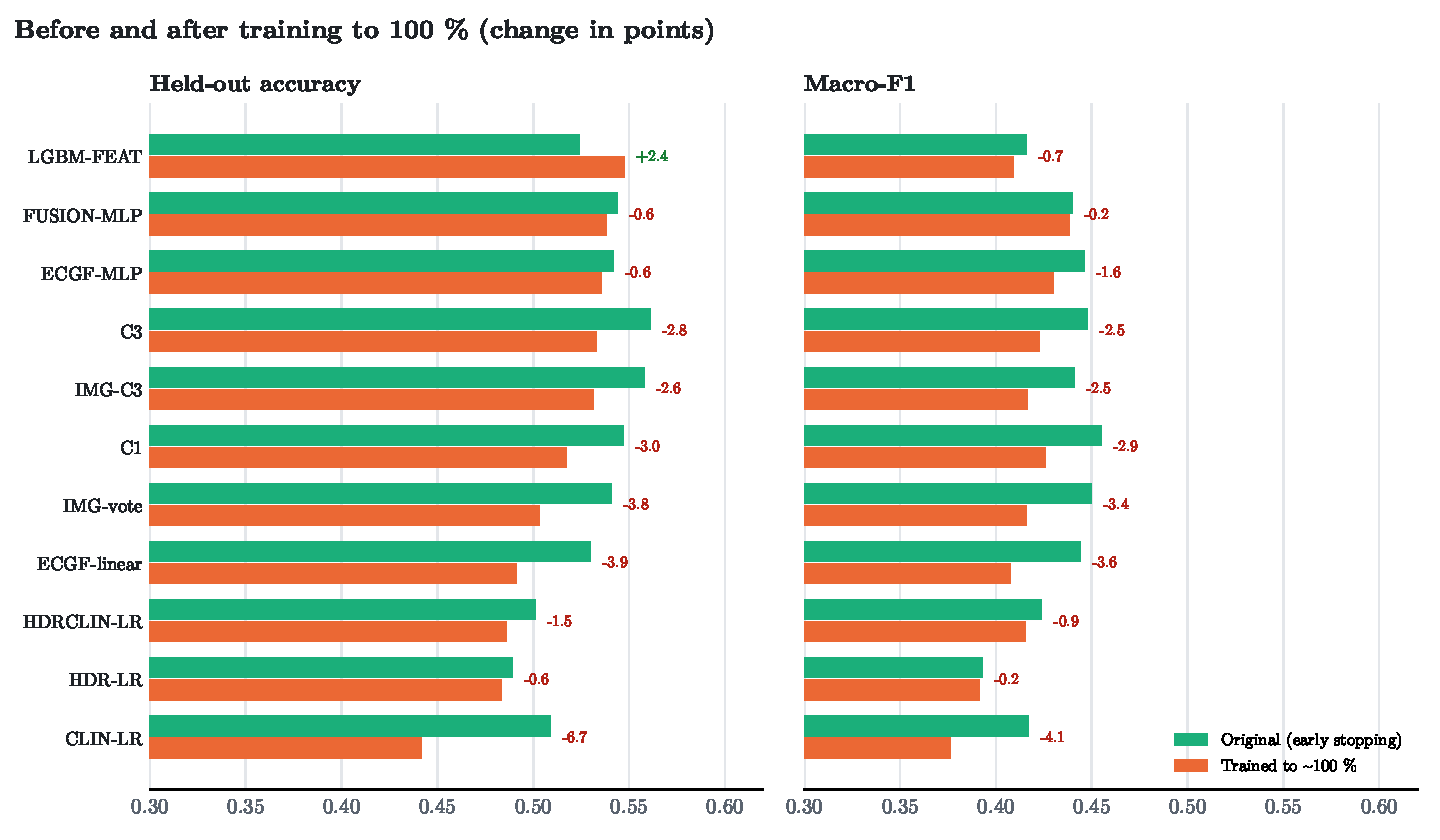
\includegraphics[width=\linewidth]{figures/fig_before_after}
\caption{Original against trained-to-100\,\% for every four-class main model; red numbers = loss in points.}
\end{figure}

\begin{figure}[H]
\centering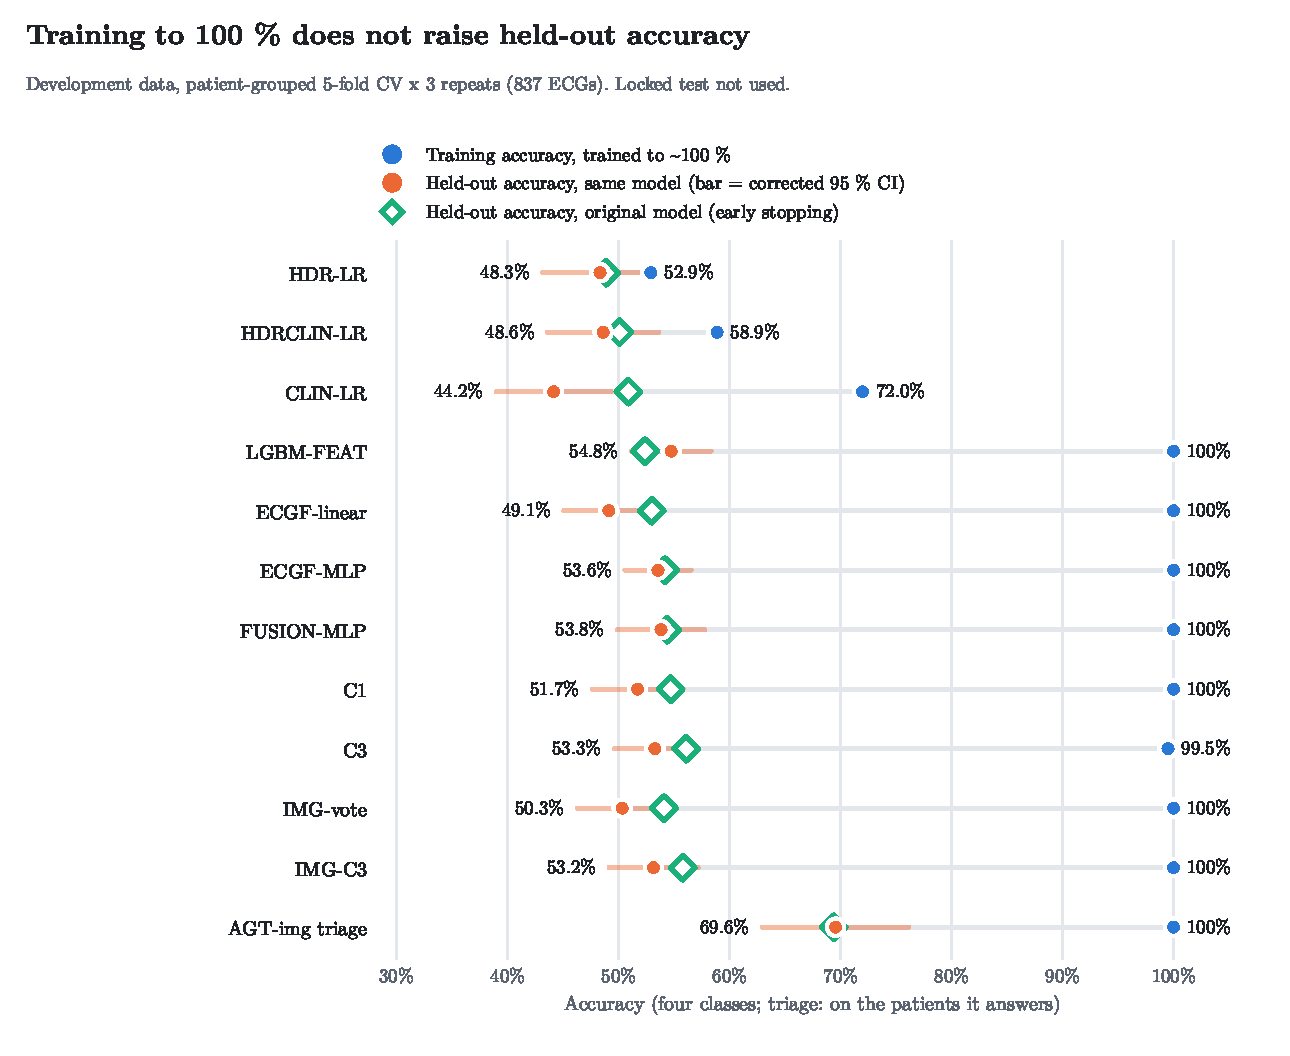
\includegraphics[width=0.86\linewidth]{figures/fig_train_vs_heldout}
\caption{Training accuracy (blue) against held-out accuracy (orange, with 95\,\% CI) and the original held-out accuracy (green).}
\end{figure}

\section{How the main models are built}
\begin{table}[htbp]
\centering
\caption{How the main models are built. ECGFounder (Net1D, 30.7 M parameters: 61 convolution and 40 linear layers in 7 stages of 20 residual blocks) is pre-trained on 10.8 million ECGs and kept frozen; only the heads are trained on the hospital ECGs. Epochs: median over the 15 folds to reach 100\,\% training accuracy; models without epochs show what replaces them.}\label{tab:main_build}
\footnotesize
\begin{tabular}{>{\raggedright\arraybackslash\hspace{0pt}}p{\dimexpr 0.120\linewidth-2\tabcolsep\relax}>{\raggedright\arraybackslash\hspace{0pt}}p{\dimexpr 0.250\linewidth-2\tabcolsep\relax}>{\raggedright\arraybackslash\hspace{0pt}}p{\dimexpr 0.350\linewidth-2\tabcolsep\relax}>{\raggedright\arraybackslash\hspace{0pt}}p{\dimexpr 0.120\linewidth-2\tabcolsep\relax}>{\raggedright\arraybackslash\hspace{0pt}}p{\dimexpr 0.160\linewidth-2\tabcolsep\relax}}
\toprule
\textbf{Model} & \textbf{Inputs} & \textbf{Layers / structure} & \textbf{Parameters} & \textbf{Epochs} \\
\midrule
HDR-LR & 16 header measurements (age, sex, rate, intervals, axes) & 1 linear layer (16 $\rightarrow$ 4) & 68 & solver (L-BFGS) \\
HDRCLIN-LR & 16 header + 28 clinical ECG features (44 inputs) & 1 linear layer (44 $\rightarrow$ 4) & 180 & solver (L-BFGS) \\
CLIN-LR & 118 image-only clinician features & 1 linear layer (118 $\rightarrow$ 4) & 476 & solver (L-BFGS) \\
LGBM-FEAT & 16 header + 403 engineered waveform features (419) & 2,000 boosting rounds $\times$ 4 classes, 31 leaves per tree & 8,000 trees & 2,000 trees \\
ECGF-linear & frozen ECGFounder embedding (1,024) & frozen backbone + 1 linear layer (1,024 $\rightarrow$ 4) & 4.1 k trained & 100 L-BFGS iter. \\
ECGF-MLP & frozen ECGFounder embedding (1,024) & frozen backbone + MLP: dropout, linear 1,024 $\rightarrow$ 64, GELU, dropout, linear 64 $\rightarrow$ 4 (2 layers); 3 seeds & 65.9 k trained & 108 \\
FUSION-MLP & 16 header + ECGFounder embedding (1,040) & MLP head as ECGF-MLP (2 linear layers); 3 seeds & 67.0 k trained & 112 \\
C1 & FUSION-MLP + ECGF-linear + HDRCLIN-LR & average of 3 members' probabilities & members & 112 (FUSION-MLP) \\
C3 & C1 & C1 + nested prior rule (one $\alpha$ chosen on inner OOF) & members + 1 & 112 (FUSION-MLP) \\
IMG-vote & ECGF-MLP + ECGF-linear (image only) & average of 2 members' probabilities & members & 108 (ECGF-MLP) \\
IMG-C3 & IMG-vote & IMG-vote + nested prior rule & members + 1 & 108 (ECGF-MLP) \\
Triage & ECGFounder + 118 clinician features $\rightarrow$ EF; IMG-C3 & ridge + LightGBM EF regressors $\rightarrow$ EF grade (3 cut-points) + margin; answers when the grade agrees with IMG-C3 & regressors + 4 & 4,000 trees \\
\bottomrule
\end{tabular}
\end{table}


\clearpage
\section{Confusion matrices}
\begin{figure}[H]
\centering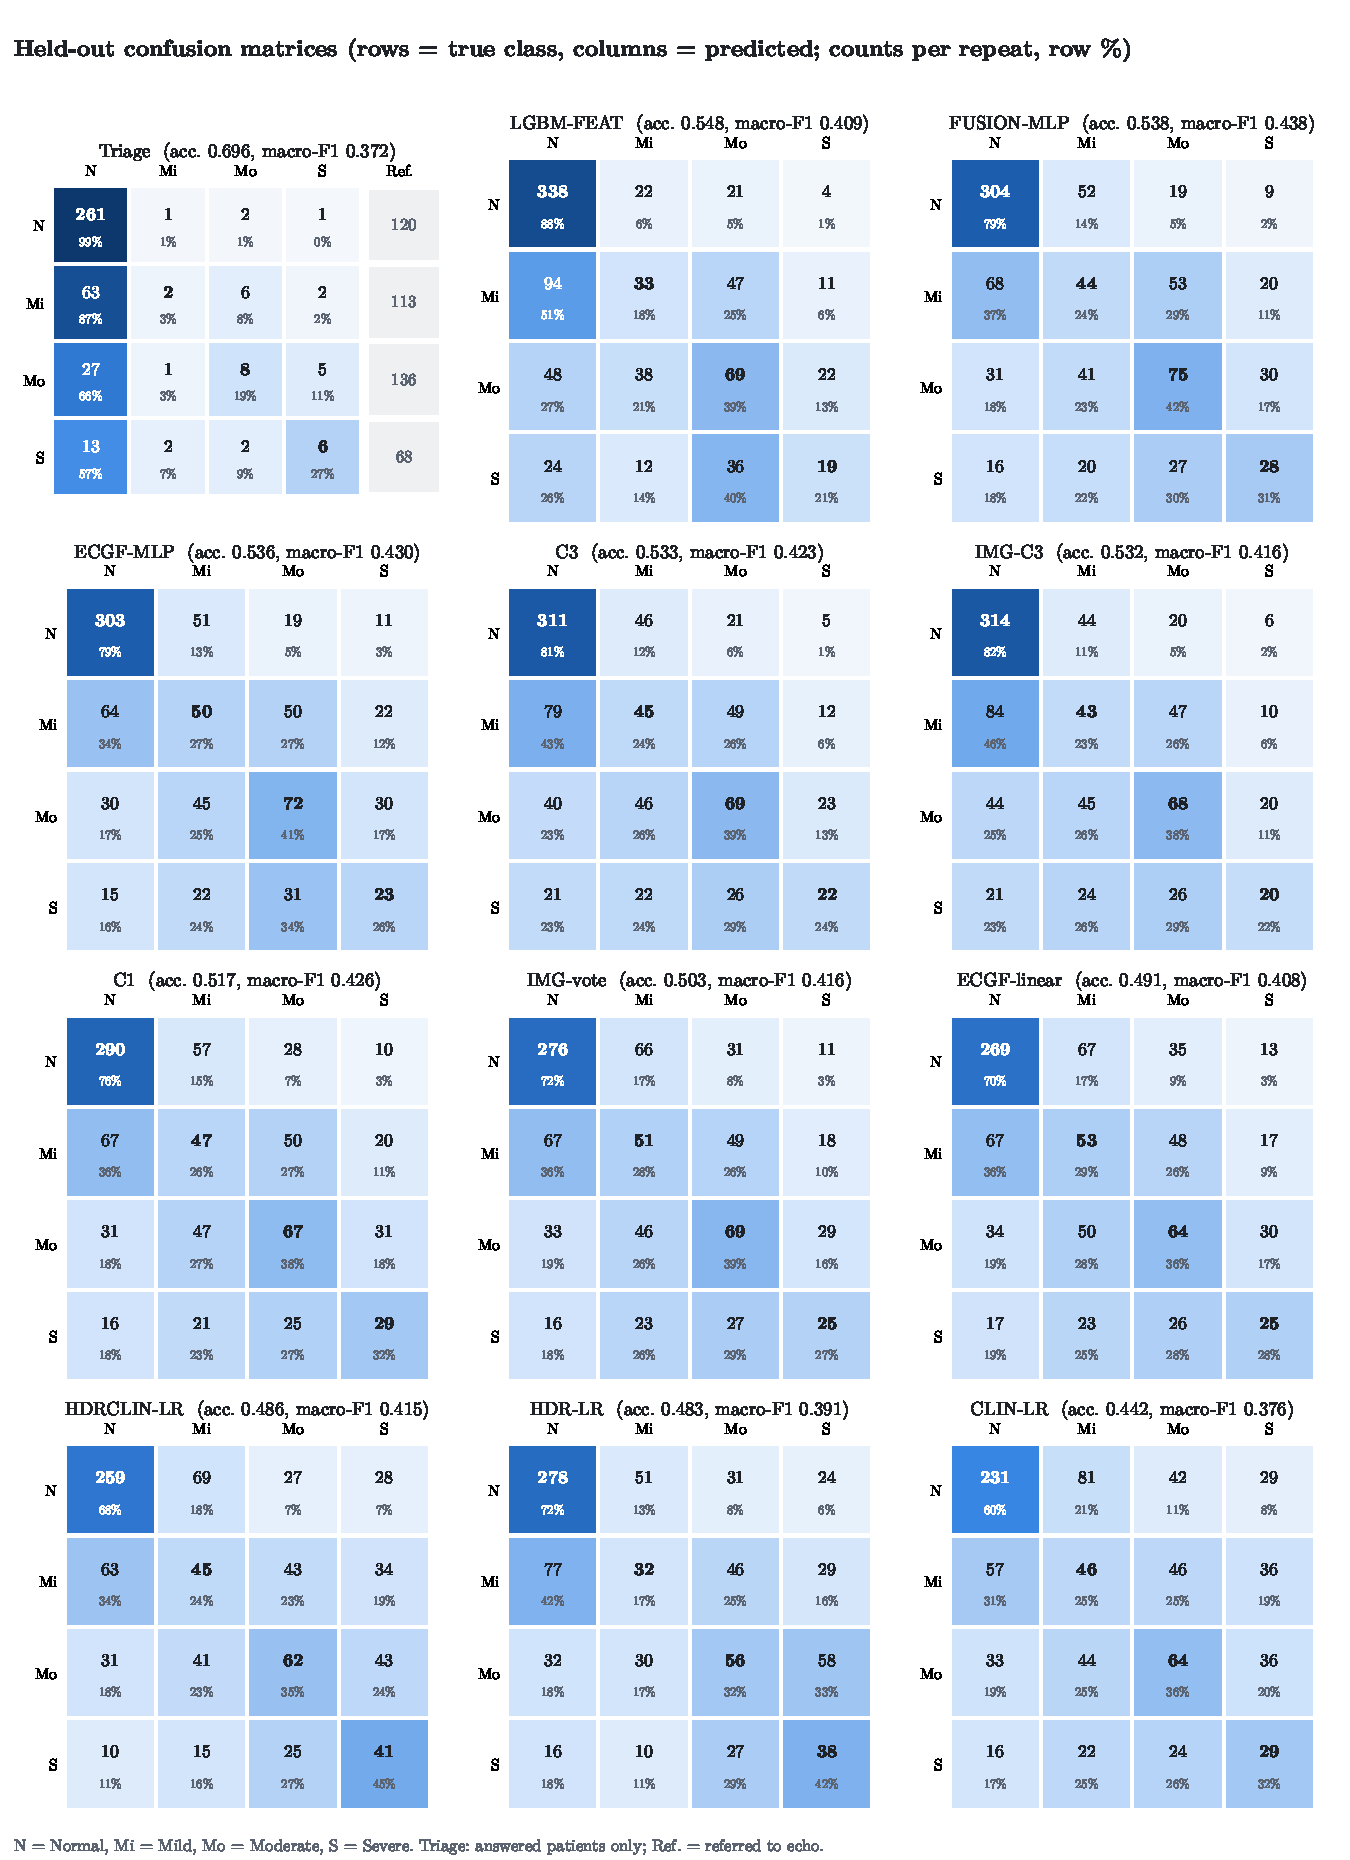
\includegraphics[width=\linewidth,height=0.80\textheight,keepaspectratio]{figures/fig_confusion}
\caption{Held-out confusion matrices of all twelve main models, ordered by accuracy. Counts are per repeat (the 837 ECGs are predicted once per repeat); colour = row percentage (recall).}
\end{figure}

\begin{figure}[H]
\centering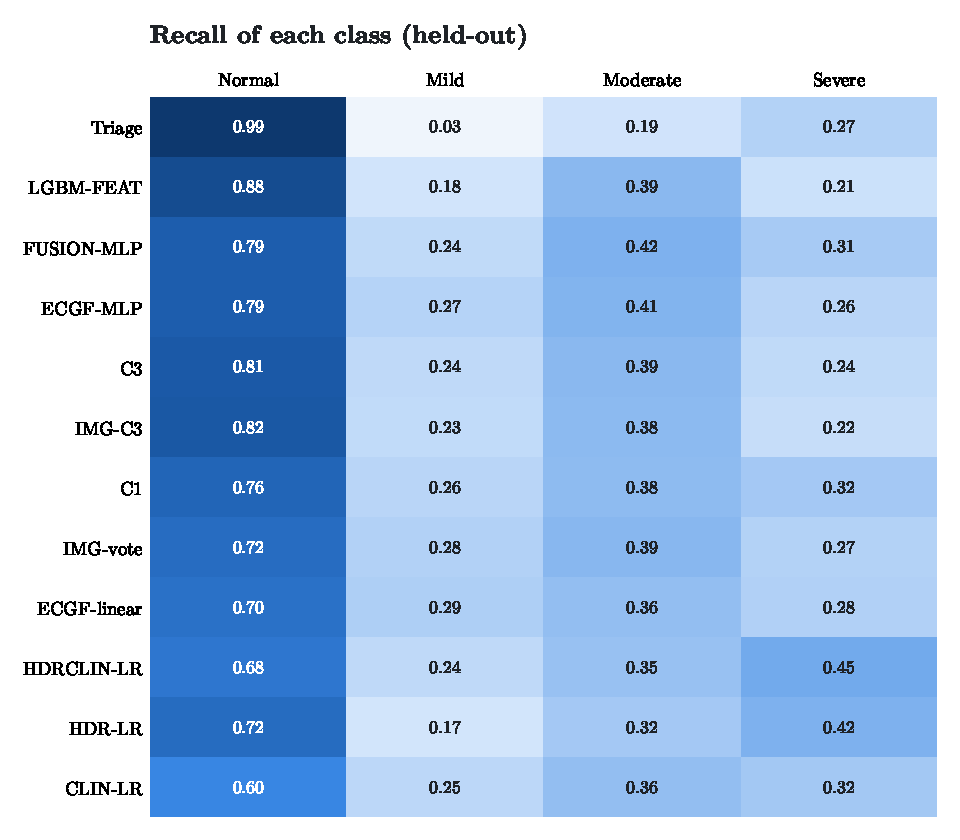
\includegraphics[width=0.72\linewidth]{figures/fig_recall}
\caption{Recall of each class. Normal is found most often; Mild is the weakest class for every model.}
\end{figure}

\section{Image and signal networks (original fixed split)}
\begin{table}[htbp]
\centering
\caption{Image and signal networks on the original fixed split (trained on 669 ECGs, validated on 168; the locked test is not loaded), ranked by validation accuracy. Best = highest validation accuracy at any epoch on the way to 100\,\%.}\label{tab:fixed}
\scriptsize
\begin{tabular}{>{\raggedright\arraybackslash\hspace{0pt}}p{\dimexpr 0.170\linewidth-2\tabcolsep\relax}>{\raggedright\arraybackslash\hspace{0pt}}p{\dimexpr 0.220\linewidth-2\tabcolsep\relax}>{\raggedright\arraybackslash\hspace{0pt}}p{\dimexpr 0.075\linewidth-2\tabcolsep\relax}>{\raggedright\arraybackslash\hspace{0pt}}p{\dimexpr 0.075\linewidth-2\tabcolsep\relax}>{\raggedright\arraybackslash\hspace{0pt}}p{\dimexpr 0.080\linewidth-2\tabcolsep\relax}>{\raggedright\arraybackslash\hspace{0pt}}p{\dimexpr 0.080\linewidth-2\tabcolsep\relax}>{\raggedright\arraybackslash\hspace{0pt}}p{\dimexpr 0.090\linewidth-2\tabcolsep\relax}>{\raggedright\arraybackslash\hspace{0pt}}p{\dimexpr 0.090\linewidth-2\tabcolsep\relax}>{\raggedright\arraybackslash\hspace{0pt}}p{\dimexpr 0.080\linewidth-2\tabcolsep\relax}}
\toprule
\textbf{Model} & \textbf{Layers} & \textbf{Params} & \textbf{Epochs} & \textbf{Train.} & \textbf{Valid.} & \textbf{Best valid.} & \textbf{Orig. valid.} & \textbf{Change} \\
\midrule
ECGFounder fine-tuned (stages 5--6) & 61 conv + 40 linear (stages 5--6 trained) + 1 FC & 30.7 M & 12 & 0.996 & 0.560 & 0.560 & 0.524 & +3.6 \\
XGBoost (waveform features) & 2,000 trees & -- & -- & 1.000 & 0.494 & -- & 0.500 & -0.6 \\
Header 0.6 + ResNet-18 0.4 & weighted average & -- & -- & 0.972 & 0.458 & -- & 0.565 & -10.7 \\
1-D SE-ResNet & 37 conv + 1 FC & 4.5 M & 32 & 0.999 & 0.435 & 0.542 & 0.482 & -4.7 \\
ECGNet & 29 conv (incl. SE) + 1 FC & 6.3 M & 21 & 0.999 & 0.435 & 0.488 & 0.476 & -4.1 \\
HOG + RBF-SVM & PCA-150 + RBF kernel & -- & -- & 1.000 & 0.423 & -- & 0.458 & -3.5 \\
ResNet-18 & 20 conv + 1 FC (18 weight layers) & 11.2 M & 24 & 0.997 & 0.423 & 0.482 & 0.524 & -10.1 \\
EfficientNet-B0 & 81 conv (16 MBConv) + 1 FC & 4.0 M & 37 & 1.000 & 0.417 & 0.512 & 0.351 & +6.6 \\
Logistic regression (header) & 1 linear layer & -- & -- & 0.674 & 0.405 & -- & 0.500 & -9.5 \\
MobileNetV3-Large & 63 conv (15 bottlenecks) + 1 FC & 4.2 M & 57 & 0.999 & 0.387 & 0.476 & 0.185 & +20.2 \\
ConvNeXt-Atto & 40 conv (12 blocks) + 1 FC & 3.4 M & 53 & 0.996 & 0.345 & 0.518 & 0.452 & -10.7 \\
\bottomrule
\end{tabular}
\end{table}

\begin{figure}[H]
\centering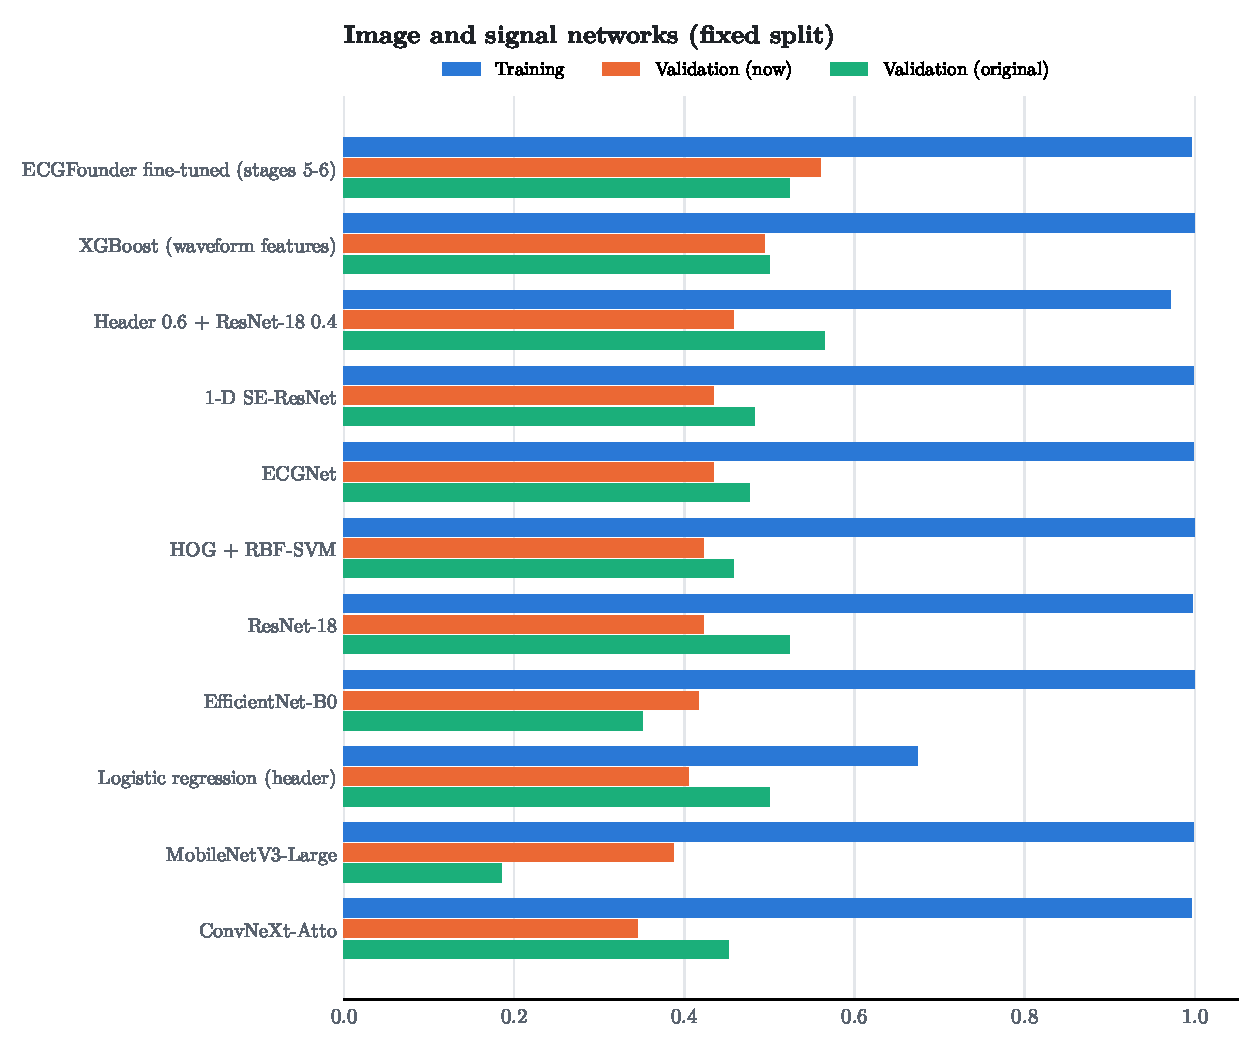
\includegraphics[width=0.86\linewidth]{figures/fig_fixed}
\caption{Training, validation and original validation accuracy of the image and signal networks.}
\end{figure}

\section{Variants of every phase}
\begin{table}[htbp]
\centering
\caption{Variants of every phase (Phases 4, 5 and 6B, development cross-validation), ranked by held-out accuracy. SUPER-TOP10-ORD: hospital-only members; its original is the same recipe on the original members (the published 0.587 also used EchoNext).}\label{tab:variants}
\footnotesize
\begin{tabular}{>{\raggedright\arraybackslash\hspace{0pt}}p{\dimexpr 0.360\linewidth-2\tabcolsep\relax}>{\raggedright\arraybackslash\hspace{0pt}}p{\dimexpr 0.100\linewidth-2\tabcolsep\relax}>{\raggedright\arraybackslash\hspace{0pt}}p{\dimexpr 0.200\linewidth-2\tabcolsep\relax}>{\raggedright\arraybackslash\hspace{0pt}}p{\dimexpr 0.080\linewidth-2\tabcolsep\relax}>{\raggedright\arraybackslash\hspace{0pt}}p{\dimexpr 0.080\linewidth-2\tabcolsep\relax}>{\raggedright\arraybackslash\hspace{0pt}}p{\dimexpr 0.090\linewidth-2\tabcolsep\relax}>{\raggedright\arraybackslash\hspace{0pt}}p{\dimexpr 0.090\linewidth-2\tabcolsep\relax}}
\toprule
\textbf{Model} & \textbf{Training acc.} & \textbf{Held-out acc. [95\,\% CI]} & \textbf{Macro-F1} & \textbf{Mild F1} & \textbf{Original} & \textbf{Change} \\
\midrule
E2 LightGBM (eng + ECGF-PCA) & 1.000 & 0.557 [0.517, 0.597] & 0.422 & 0.208 & 0.544 & +1.3 \\
ENH-vote & 1.000 & 0.549 [0.513, 0.585] & 0.418 & 0.223 & 0.569 & -2.0 \\
ULT M9 kNN (k 15, distance) & 1.000 & 0.546 [0.520, 0.571] & 0.382 & 0.172 & -- & -- \\
E6 signal-quality gating & 0.988 & 0.542 [0.500, 0.583] & 0.441 & 0.258 & 0.546 & -0.4 \\
E1 MLP, all feature families & 1.000 & 0.542 [0.504, 0.579] & 0.442 & 0.259 & 0.554 & -1.2 \\
ULT M10 gradient boosting & 1.000 & 0.540 [0.496, 0.585] & 0.409 & 0.223 & -- & -- \\
E4 hierarchical MLP & 0.999 & 0.540 [0.517, 0.563] & 0.433 & 0.250 & 0.567 & -2.7 \\
SUPER-TOP10-ORD without EchoNext & 0.783 & 0.539 [0.509, 0.570] & 0.400 & 0.196 & 0.565 & -2.6 \\
ULT-stack (no EchoNext) & 0.794 & 0.537 [0.500, 0.574] & 0.409 & 0.231 & 0.571 & -3.4 \\
Multitask MLP (class + EF) & 1.000 & 0.536 [0.496, 0.577] & 0.434 & 0.258 & 0.546 & -1.0 \\
HIER (two-stage) & 1.000 & 0.535 [0.488, 0.582] & 0.426 & 0.217 & 0.570 & -3.5 \\
E7 mixup MLP & 1.000 & 0.534 [0.499, 0.570] & 0.434 & 0.263 & 0.552 & -1.8 \\
E3 stacking (LR, balanced) & 0.826 & 0.532 [0.487, 0.576] & 0.418 & 0.172 & 0.546 & -1.4 \\
E3 weighted average & 0.985 & 0.530 [0.480, 0.581] & 0.428 & 0.244 & 0.547 & -1.7 \\
ENH M5 LR on HIER inputs & 1.000 & 0.501 [0.450, 0.553] & 0.417 & 0.286 & 0.543 & -4.2 \\
ULT M8 LR multi-scale ECGF & 1.000 & 0.496 [0.459, 0.532] & 0.399 & 0.246 & -- & -- \\
ENH M2 synthetic 10-s $\rightarrow$ ECGFounder & 1.000 & 0.489 [0.439, 0.539] & 0.404 & 0.280 & 0.528 & -3.9 \\
ENH M6 EF ridge $\rightarrow$ bands & 0.557 & 0.477 [0.458, 0.496] & 0.257 & 0.004 & 0.534 & -5.7 \\
ENH M4 MiniRocket & 1.000 & 0.469 [0.423, 0.515] & 0.390 & 0.229 & 0.504 & -3.5 \\
ENH M3 median-beat shape & 1.000 & 0.412 [0.358, 0.466] & 0.345 & 0.225 & 0.467 & -5.5 \\
ULT M12 zone LR & 0.624 & 0.349 [0.302, 0.396] & 0.278 & 0.311 & -- & -- \\
\bottomrule
\end{tabular}
\end{table}

\begin{figure}[H]
\centering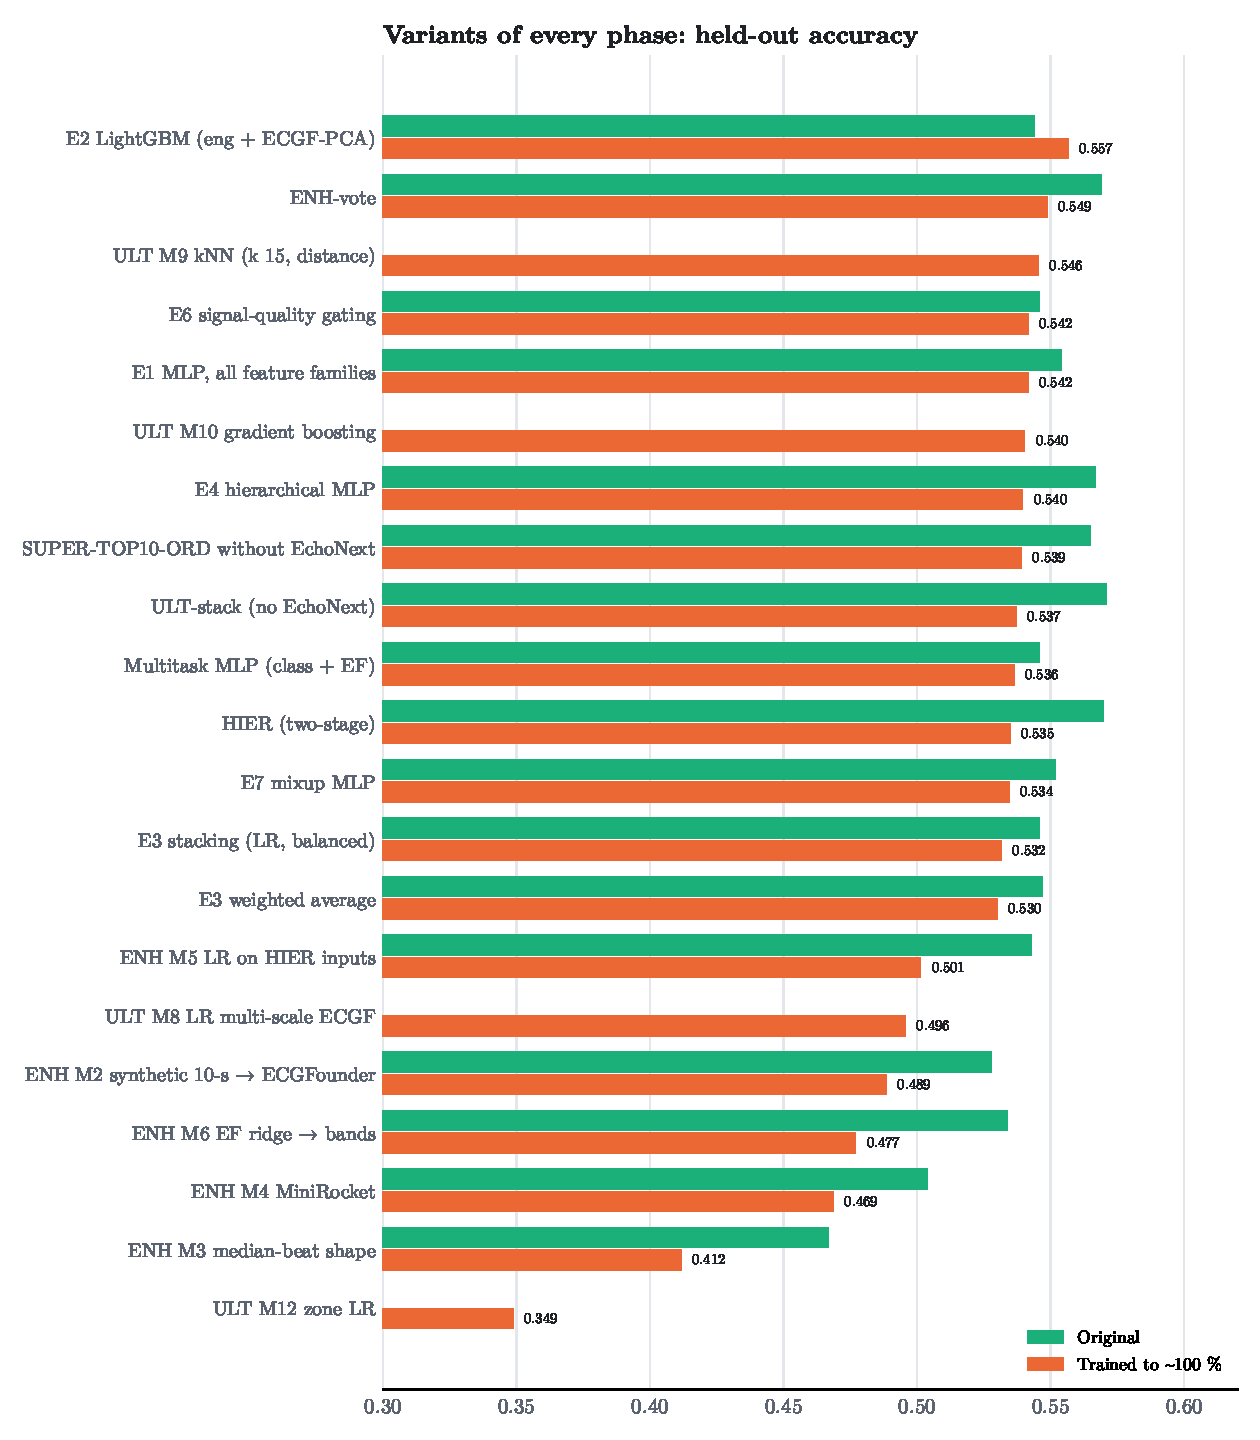
\includegraphics[width=0.86\linewidth]{figures/fig_variants}
\caption{Variants of Phases 4, 5 and 6B: held-out accuracy of the original and of the model trained to (nearly) 100\,\%.}
\end{figure}

\section{Label-quality studies}
\begin{table}[htbp]
\centering
\caption{Label-quality studies with the C3 recipe trained to (nearly) 100\,\%, scored on the same subsets as report Table 4.7, ranked by accuracy. Epochs: median of the FUSION-MLP member.}\label{tab:labels}
\footnotesize
\begin{tabular}{>{\raggedright\arraybackslash\hspace{0pt}}p{\dimexpr 0.300\linewidth-2\tabcolsep\relax}>{\raggedright\arraybackslash\hspace{0pt}}p{\dimexpr 0.150\linewidth-2\tabcolsep\relax}>{\raggedright\arraybackslash\hspace{0pt}}p{\dimexpr 0.080\linewidth-2\tabcolsep\relax}>{\raggedright\arraybackslash\hspace{0pt}}p{\dimexpr 0.110\linewidth-2\tabcolsep\relax}>{\raggedright\arraybackslash\hspace{0pt}}p{\dimexpr 0.110\linewidth-2\tabcolsep\relax}>{\raggedright\arraybackslash\hspace{0pt}}p{\dimexpr 0.110\linewidth-2\tabcolsep\relax}>{\raggedright\arraybackslash\hspace{0pt}}p{\dimexpr 0.100\linewidth-2\tabcolsep\relax}}
\toprule
\textbf{Study} & \textbf{Scored on} & \textbf{Epochs} & \textbf{Training acc.} & \textbf{Accuracy} & \textbf{Original} & \textbf{Change} \\
\midrule
NFS: noise-free, Severe kept & 264 clean & 44 & 0.985 & 0.694 & 0.702 & -0.8 \\
NF: noise-free & 264 clean & 45 & 1.000 & 0.673 & 0.683 & -1.0 \\
CLEAR: no border ECGs & 582 clear-cut & 104 & 0.993 & 0.670 & 0.668 & +0.2 \\
MMCLEAN: suspect Mild/Mod. dropped & 620 kept & 95 & 0.978 & 0.669 & 0.672 & -0.3 \\
HC30: reliable links only & 395 reliable & 52 & 1.000 & 0.583 & 0.594 & -1.1 \\
VER: 15 labels corrected & all 837 & 132 & 0.986 & 0.537 & 0.565 & -2.8 \\
\bottomrule
\end{tabular}
\end{table}


\section{Top-3 ensembles with EchoNext (owner's laptop)}\label{sec:echonext}
\begin{table}[htbp]
\centering
\caption{Top-3 ensembles retrained to (nearly) 100\,\% with EchoNext on the owner's laptop (numbers as reported by that session; EchoNext data never left the laptop).}\label{tab:echonext}
\small
\begin{tabular}{>{\raggedright\arraybackslash\hspace{0pt}}p{\dimexpr 0.360\linewidth-2\tabcolsep\relax}>{\raggedright\arraybackslash\hspace{0pt}}p{\dimexpr 0.140\linewidth-2\tabcolsep\relax}>{\raggedright\arraybackslash\hspace{0pt}}p{\dimexpr 0.240\linewidth-2\tabcolsep\relax}>{\raggedright\arraybackslash\hspace{0pt}}p{\dimexpr 0.130\linewidth-2\tabcolsep\relax}>{\raggedright\arraybackslash\hspace{0pt}}p{\dimexpr 0.130\linewidth-2\tabcolsep\relax}}
\toprule
\textbf{Model} & \textbf{Training acc.} & \textbf{Held-out acc. [95\,\% CI]} & \textbf{Original} & \textbf{Change} \\
\midrule
SUPER-TOP10-ORD (best for 50s) & 0.748 & 0.558 [0.530, 0.587] & 0.587 & -2.9 \\
SUPER (greedy) & 0.790 & 0.552 [0.507, 0.596] & 0.583 & -3.1 \\
STAGED-4 (pool X) & 0.722 & 0.548 [0.516, 0.581] & 0.585 & -3.7 \\
\bottomrule
\end{tabular}
\end{table}

\begin{table}[htbp]
\centering
\caption{Members of the three ensembles (laptop run), ranked by hospital held-out accuracy. $^{\ddagger}$ Two-class task. $^{\circ}$ Trained on EchoNext only: training and validation accuracy on EchoNext, held-out accuracy on the hospital ECGs (H / plain input). -- = not reported.}\label{tab:echonext_members}
\footnotesize
\begin{tabular}{>{\raggedright\arraybackslash\hspace{0pt}}p{\dimexpr 0.460\linewidth-2\tabcolsep\relax}>{\raggedright\arraybackslash\hspace{0pt}}p{\dimexpr 0.160\linewidth-2\tabcolsep\relax}>{\raggedright\arraybackslash\hspace{0pt}}p{\dimexpr 0.180\linewidth-2\tabcolsep\relax}>{\raggedright\arraybackslash\hspace{0pt}}p{\dimexpr 0.200\linewidth-2\tabcolsep\relax}}
\toprule
\textbf{Member} & \textbf{Training acc.} & \textbf{EchoNext validation} & \textbf{Hospital held-out acc.} \\
\midrule
EN-MiMo-GBM (Mild vs Moderate)$^{\ddagger\circ}$ & 1.000 & 0.694 & 0.586 \\
EN-MiMo-LR (Mild vs Moderate)$^{\ddagger\circ}$ & 1.000 & 0.604 & 0.577 \\
H-MiMo-GBM (Mild vs Moderate)$^{\ddagger}$ & 1.000 & -- & 0.569 \\
H-TAB-GBM & 1.000 & -- & 0.548 \\
M9 & 1.000 & -- & 0.546 \\
H-X-GBM & 1.000 & -- & 0.546 \\
EN-gbm-X$^{\circ}$ & 1.000 & 0.756 & 0.539 \\
M10 & 1.000 & -- & 0.539 \\
ECGF-MLP & 0.996 & -- & 0.536 \\
EN-gbm (H / plain)$^{\circ}$ & 1.000 & 0.756 & 0.522 / 0.522 \\
M5 & 1.000 & -- & 0.507 \\
PIX-ZS (CNN on GPU)$^{\circ}$ & 0.999 & 0.725 & 0.505 \\
ECGF-lin & 1.000 & -- & 0.498 \\
EN-cls-all-X$^{\circ}$ & 0.996 & 0.694 & 0.497 \\
M8 & 1.000 & -- & 0.496 \\
PIX-ZS-band$^{\circ}$ & 0.929 & 0.642 & 0.492 \\
EN-cls-all (H / plain)$^{\circ}$ & 0.999 & 0.673 & 0.490 / 0.464 \\
EF-band & -- & -- & 0.479 \\
EN-cls$^{\circ}$ & 1.000 & 0.663 & 0.479 \\
EN-band$^{\circ}$ & 0.781 & 0.520 & 0.479 \\
M6 (EF bands) & 0.557 & -- & 0.477 \\
H-TAB-LR & 1.000 & -- & 0.473 \\
EN-band-all (H / plain)$^{\circ}$ & 0.820 & 0.525 & 0.458 / 0.465 \\
EN-mu-mid$^{\circ}$ & 0.999 & 0.463 & 0.409 \\
M12 & 1.000 & -- & 0.346 \\
\bottomrule
\end{tabular}
\end{table}


\section{Training accuracy of all models}
\begin{small}
\begin{longtable}{>{\raggedright\arraybackslash}p{10.2cm}>{\raggedright\arraybackslash}p{2.8cm}>{\raggedright\arraybackslash}p{2.2cm}}
\caption{Training accuracy and epochs of every model, sorted from highest to lowest within each group.}\label{tab:alltrain}\\
\toprule \textbf{Model} & \textbf{Epochs (median)} & \textbf{Training accuracy} \\ \midrule \endfirsthead
\toprule \textbf{Model} & \textbf{Epochs (median)} & \textbf{Training accuracy} \\ \midrule \endhead
\bottomrule \endfoot
\multicolumn{3}{l}{\textbf{(a) Main models, development cross-validation}} \\
LightGBM on engineered features (LGBM-FEAT) & 2,000 trees & 1.000 \\
ECGFounder linear head (ECGF-linear) & 100 iter. & 1.000 \\
ECGFounder MLP head (ECGF-MLP) & 108 & 1.000 \\
Header + ECGFounder MLP fusion (FUSION-MLP) & 112 & 1.000 \\
C1: vote ensemble & 112$^{b}$ & 1.000 \\
IMG-vote: image-only vote & 108$^{c}$ & 1.000 \\
IMG-C3: image-only vote + prior rule & 108$^{c}$ & 1.000 \\
Image-only triage (AGT-img)$^{\dagger}$ & 4,000 trees & 1.000 \\
MMCLEAN selective$^{\dagger\,*}$ & n/r & 0.999 \\
C3: vote + nested prior rule & 112$^{b}$ & 0.995 \\
Image-only clinician features, logistic regression (CLIN-LR) & solver & 0.720 \\
Header + clinical features, logistic regression (HDRCLIN-LR) & solver & 0.589 \\
Header measurements, logistic regression (HDR-LR) & solver & 0.529 \\
\midrule
\multicolumn{3}{l}{\textbf{(b) Variants of every phase, development cross-validation}} \\
E1 MLP, header + ECGFounder + feature families & 64 & 1.000 \\
E2 LightGBM, features + ECGFounder PCA & 2,000 trees & 1.000 \\
E7 mixup MLP & 144 & 1.000 \\
Multitask MLP (class + EF) & 131 & 1.000 \\
HIER two-stage & 108$^{c}$ & 1.000 \\
ENH M2 synthetic 10-s ECG $\rightarrow$ ECGFounder & solver & 1.000 \\
ENH M3 median-beat shape & solver & 1.000 \\
ENH M4 MiniRocket & solver & 1.000 \\
ENH M5 logistic regression & solver & 1.000 \\
ENH-vote & 108$^{c}$ & 1.000 \\
ULT M9 kNN & none & 1.000 \\
ULT M10 gradient boosting & 2,000 iter. & 1.000 \\
ULT M8 multi-scale ECGFounder LR & solver & 1.000 \\
E4 hierarchical MLP & 52 / 39 & 0.999 \\
E6 signal-quality gating & 112$^{b}$ & 0.988 \\
E3 weighted average of the C1 members & 112$^{b}$ & 0.985 \\
E3 stacking (logistic meta-learner) & 112$^{b}$ & 0.826 \\
ULT-stack & 108$^{c}$ & 0.794 \\
SUPER-TOP10-ORD, hospital members only & 108$^{c}$ & 0.783 \\
ULT M12 zone LR & solver & 0.624 \\
ENH M6 EF ridge $\rightarrow$ bands & exact & 0.557 \\
\midrule
\multicolumn{3}{l}{\textbf{(c) Label-quality studies (C3 recipe)}} \\
HC30: reliable links only & 52$^{b}$ & 1.000 \\
NF: noise-free training & 45$^{b}$ & 1.000 \\
CLEAR: without border ECGs & 104$^{b}$ & 0.993 \\
VER: corrected labels & 132$^{b}$ & 0.986 \\
NFS: noise-free training, Severe kept & 44$^{b}$ & 0.985 \\
MMCLEAN: suspect Mild or Moderate labels dropped & 95$^{b}$ & 0.978 \\
\midrule
\multicolumn{3}{l}{\textbf{(d) Image and signal networks, original fixed split}} \\
EfficientNet-B0 & 37 & 1.000 \\
HOG + RBF-SVM & solver & 1.000 \\
XGBoost (waveform features) & 2,000 trees & 1.000 \\
MobileNetV3-Large & 57 & 0.999 \\
1-D SE-ResNet & 32 & 0.999 \\
ECGNet & 21 & 0.999 \\
ResNet-18 & 24 & 0.997 \\
ECGFounder fine-tuned (stages 5--6) & 12 & 0.996 \\
ConvNeXt-Atto & 53 & 0.996 \\
Header 0.6 + ResNet-18 0.4 & 24 (ResNet-18) & 0.972 \\
Logistic regression (header) & solver & 0.674 \\
\midrule
\multicolumn{3}{l}{\textbf{(e) Laptop run with EchoNext$^{*}$ (top-3 ensembles and their members)}} \\
ECGF-lin & n/r & 1.000 \\
M5 & n/r & 1.000 \\
M8 & n/r & 1.000 \\
M9 & n/r & 1.000 \\
M10 & n/r & 1.000 \\
M12 & n/r & 1.000 \\
H-TAB-LR & n/r & 1.000 \\
H-TAB-GBM & n/r & 1.000 \\
H-X-GBM & n/r & 1.000 \\
H-MiMo-GBM (Mild vs Moderate)$^{\ddagger}$ & n/r & 1.000 \\
EN-cls$^{\circ}$ & n/r & 1.000 \\
EN-gbm (H / plain)$^{\circ}$ & n/r & 1.000 \\
EN-gbm-X$^{\circ}$ & n/r & 1.000 \\
EN-MiMo-LR (Mild vs Moderate)$^{\ddagger\,\circ}$ & n/r & 1.000 \\
EN-MiMo-GBM (Mild vs Moderate)$^{\ddagger\,\circ}$ & n/r & 1.000 \\
EN-cls-all (H / plain)$^{\circ}$ & n/r & 0.999 \\
PIX-ZS (CNN on GPU)$^{\circ}$ & n/r & 0.999 \\
EN-mu-mid$^{\circ}$ & n/r & 0.999 \\
ECGF-MLP & n/r & 0.996 \\
EN-cls-all-X$^{\circ}$ & n/r & 0.996 \\
PIX-ZS-band$^{\circ}$ & n/r & 0.929 \\
EN-band-all (H / plain)$^{\circ}$ & n/r & 0.820 \\
SUPER (greedy) & n/r & 0.790 \\
EN-band$^{\circ}$ & n/r & 0.781 \\
SUPER-TOP10-ORD (best for 50s) & n/r & 0.748 \\
STAGED-4 (pool X) & n/r & 0.722 \\
M6 (EF bands) & n/r & 0.557 \\
EF-band & n/r & --$^{\S}$ \\

\end{longtable}
\end{small}

{\footnotesize Epochs: median over the 15 folds; solver / trees / iter. = models not trained in epochs; $^{b}$ epochs of the neural member FUSION-MLP; $^{c}$ epochs of the neural member ECGF-MLP. $^{\dagger}$ Selective model: training accuracy on the patients it answers. $^{\ddagger}$ Two-class task (Mild vs Moderate). $^{\circ}$ Trained on EchoNext only (training accuracy on EchoNext). $^{*}$ Numbers from the owner's other / laptop session; n/r = not reported. $^{\S}$ Not visible in the shared screenshot. Logistic regressions on few inputs cannot reach 1.000; combiners whose decision rule is tuned on cross-validated member outputs stay below 1.000 by design.\par}

\section{Where to stop training}
\begin{figure}[H]
\centering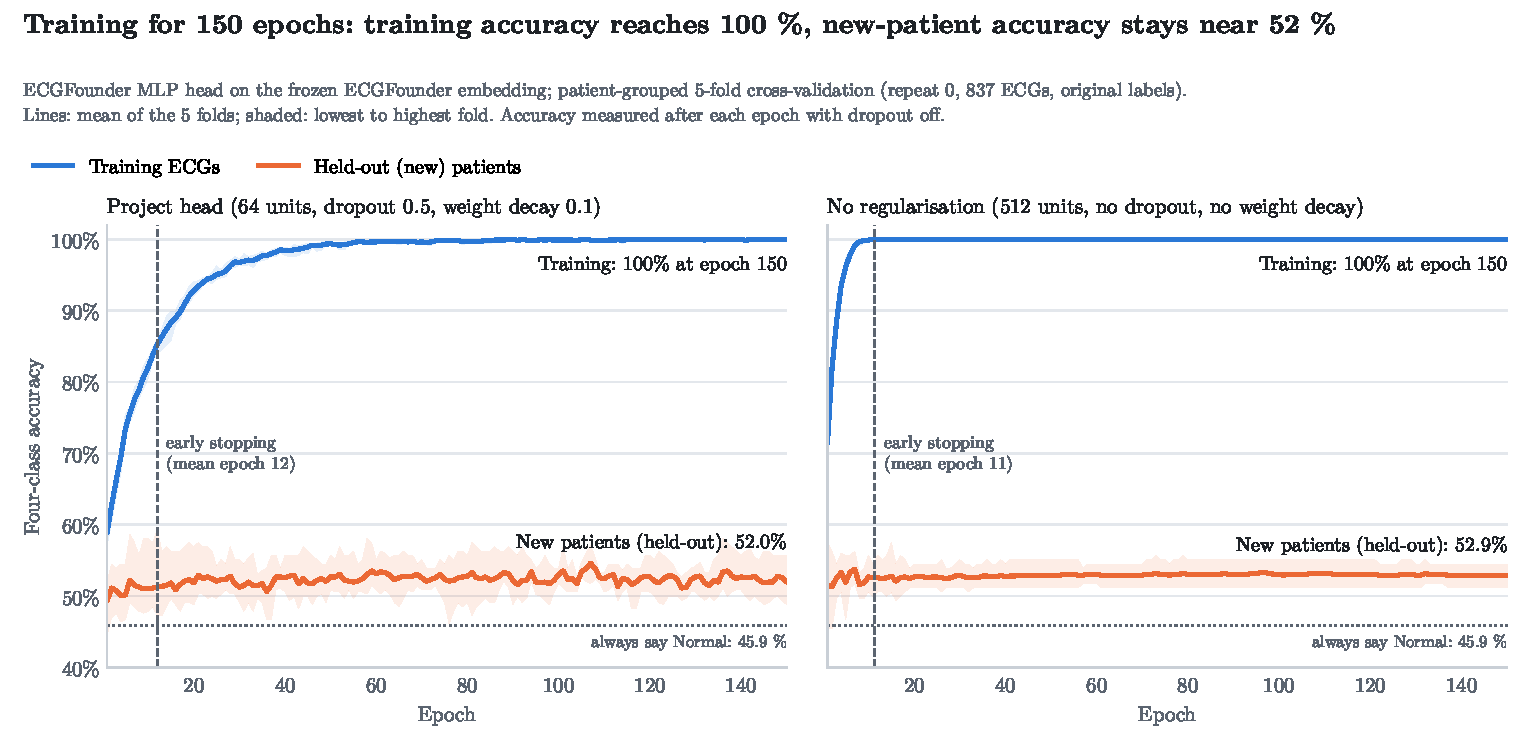
\includegraphics[width=\linewidth]{figures/fig_epochs150}
\caption{ECGFounder MLP head trained for 150 epochs: training accuracy reaches 100\,\% while held-out accuracy stays at about 0.52. The dashed line marks the early-stopping epoch.}
\end{figure}
Training to 100\,\% memorises the 670 training ECGs of each fold, including their label noise; that detail does not exist in new patients. The right stopping point is where accuracy on unseen data stops improving (inner-validation early stopping), at a training accuracy of about 0.60--0.85, and the held-out accuracy is the number to report.
\end{document}
